% !TEX root = main.tex
% CVPR 2025 Paper Template; see https://github.com/cvpr-org/author-kit

\documentclass[10pt,twocolumn,letterpaper]{article}

%%%%%%%%% PAPER TYPE  - PLEASE UPDATE FOR FINAL VERSION
% \usepackage{cvpr}              % To produce the CAMERA-READY version
% \usepackage[review]{cvpr}      % To produce the REVIEW version
\usepackage[pagenumbers]{cvpr} % To force page numbers, e.g. for an arXiv version

% Import additional packages in the preamble file, before hyperref
%
% --- inline annotations
%
\newcommand{\red}[1]{{\color{red}#1}}
\newcommand{\todo}[1]{{\color{red}#1}}
\newcommand{\TODO}[1]{\textbf{\color{red}[TODO: #1]}}
% --- disable by uncommenting  
% \renewcommand{\TODO}[1]{}
% \renewcommand{\todo}[1]{#1}
\usepackage{amsthm}
\usepackage{graphicx}
\usepackage{animate}
\newcommand{\Var}{\textup{Var}}
\newcommand{\Cov}{\textup{Cov}}
\newcommand{\bE}{\mathbb{E}}
\newtheorem{proposition}{Proposition}
\newtheorem{example}{Example}


% It is strongly recommended to use hyperref, especially for the review version.
% hyperref with option pagebackref eases the reviewers' job.
% Please disable hyperref *only* if you encounter grave issues, 
% e.g. with the file validation for the camera-ready version.
%
% If you comment hyperref and then uncomment it, you should delete *.aux before re-running LaTeX.
% (Or just hit 'q' on the first LaTeX run, let it finish, and you should be clear).
\definecolor{cvprblue}{rgb}{0.21,0.49,0.74}
\usepackage[pagebackref,breaklinks,colorlinks,allcolors=cvprblue]{hyperref}
\usepackage{comment}

%%%%%%%%% PAPER ID  - PLEASE UPDATE
\def\paperID{13930} % *** Enter the Paper ID here
\def\confName{CVPR}
\def\confYear{2025}

%%%%%%%%% TITLE - PLEASE UPDATE
\title{MotionV2V: Editing Motion in a Video}

%%%%%%%%% AUTHORS - PLEASE UPDATE
\author{
  Ryan Burgert$^{1,2}$ ~~~~~~~ Charles Herrmann$^{1}$ ~~~~~~~ Forrester Cole$^{1}$ ~~~~~~~ Michael S Ryoo$^{2}$ \\  Neal Wadhwa$^{1}$ ~~~~~~~ Andrey Voynov$^{1}$ ~~~~~~~ Nataniel Ruiz$^{1}$\\
  \\
  $^{1}$Google\;\;\;\;   $^{2}$Stony Brook University
}

\begin{document}
\maketitle

\ignore{
\twocolumn[{
\renewcommand\twocolumn[1][]{#1}
\maketitle
\begin{center}
    \centering
    \vspace*{-.6cm}
    % \includegraphics[width=0.8\textwidth]{MainDemoFigure.pdf}
    \vspace*{-.3cm}
    \captionof{figure}{Our method can edit videos in a true sense, where content is preserved but motion is changed. Above we show some practical applications.}
\label{fig:teaser}
\end{center}
}]

\begin{figure}[!h]
    \centering
    % \includegraphics[width=1\linewidth]{MotionEditsMainIdea.pdf}
    \caption{Conceptual overview of our motion editing approach. Users provide an input video along with source motion tracks (colored dots connected by lines, extracted from the input) and target motion tracks (user-specified desired motion). Lines indicate point trajectories while dot presence/absence indicates visibility. Our diffusion model generates an output video matching the target motion. The method supports iterative editing: outputs can become inputs for subsequent edits, enabling complex sequential motion changes.}
    \label{fig:concept_overview}
    \vspace{-10pt}
\end{figure}
}

\begin{abstract}

Generative modeling aims to transform random noise into structured outputs. In this work, we enhance video diffusion models by allowing motion control via structured latent noise sampling. This is achieved by just a change in data: we pre-process training videos to yield structured noise. Consequently, our method is agnostic to diffusion model design, requiring no changes to model architectures or training pipelines. Specifically, we propose a novel noise warping algorithm, fast enough to run in real time, that replaces random temporal Gaussianity with correlated warped noise derived from optical flow fields, while preserving the spatial Gaussianity. The efficiency of our algorithm enables us to fine-tune modern video diffusion base models using warped noise with minimal overhead, and provide a one-stop solution for a wide range of user-friendly motion control: local object motion control, global camera movement control, and motion transfer. The harmonization between temporal coherence and spatial Gaussianity in our warped noise leads to effective motion control while maintaining per-frame pixel quality. Extensive experiments and user studies demonstrate the advantages of our method, making it a robust and scalable approach for controlling motion in video diffusion models. Video results are available on our \href{https://eyeline-research.github.io/Go-with-the-Flow/}{webpage}; source code and model checkpoints are available on \href{https://github.com/Eyeline-Research/Go-with-the-Flow}{GitHub}.

\end{abstract}
\section{Introduction}
\label{locVLM_sec:intro}

Holistic visual understanding requires learning beyond simply content of an image to encompass awareness on spatial locations of objects and their relations \cite{marr1982vision}. In the context of visual question answering (VQA), such spatial awareness allows better reasoning involving structural and contextual information contained within an image \cite{chen2023shikra}.

Since the introduction of powerful large-language models (LLMs) such as GPT-3 \cite{brown2020language}, Chat-GPT \cite{gpt4}, Vicuna \cite{vicuna2023}, and LLaMA~\citep{touvron2023llama,touvron2023llama2} that are capable of human style conversation, their visual counterparts such as BLIP-2 \cite{li2023blip}, LLaVA \cite{liu2023visual} have enabled novel tasks within the vision modality. However, despite their \cite{li2023blip,liu2023visual} highly generic visual understanding, these models exhibit poor language-based spatial reasoning \cite{chen2023shikra}. In fact, they fail at simple tasks such as distinguishing whether an object lies to the left or right of another object (see \cref{locvlm_tbl:spatial_icl}). 
% half of the image

\begin{figure}[t]
\centering

\includegraphics[width=.5\linewidth]{figures__intro1.png}\\
\texttt{man with blonde hair in blue shirt and brown pants}

\includegraphics[width=.5\linewidth]{figures__intro2.png}\\
\texttt{bald man wearing glasses with white shirt and black pants}

\caption{\textbf{Zero-Shot Segmentation with phrases}:  We highlight the ability of \modelname to ground complex language prompts onto an image with no segmentation specific training. An off-the-shelf diffusion model is used with only an inference time optimization technique to generate these segmentations. If you look closely, you'll notice the bald man's arms are segmented - but are not visible in the photo! Peekaboo has fairly strong shape priors.}
\label{fig:intro}
\end{figure}


In the case of contrastive language image models (such as CLIP \cite{radford2021learning}, ALIGN \cite{Jia2021ScalingUV}), recent works explore how injecting explicit spatial awareness \cite{Zhang2023AssociatingSG,Luo2022SegCLIPPA,Mukhoti2022OpenVS,Ranasinghe2022PerceptualGI} can enable more holistic visual understanding. In fact, \cite{Ranasinghe2022PerceptualGI} shows how such improved spatial awareness benefits model robustness in adversarial domains. 
This raises the question of how generative language image models, particularly those connecting LLMs to visual encoders \cite{li2023blip,liu2023visual} can benefit from such spatial awareness specific training. We refer to models of this category that generate textual outputs given joint image-text inputs (e.g. \cite{li2023blip,liu2023visual}) as visual-LLMs (V-LLMs). 

In this work, we explore location specific instruction fine-tuning objectives that explicitly enforce V-LLMs to meaningfully process and generate textual image-space coordinates. We hypothesize that such training would lead to improved spatial awareness in these V-LLMs, therein improving performance on VQA tasks. To this end, we propose three instruction fine-tuning objectives that unify location representation with natural language. We also explore optimal representation forms for image-space locations and how pseudo-data generation can be leveraged for efficient scaling of our framework. We name our resulting model as LocVLM.  

While the idea of adapting V-LLMs to perform localization related tasks (e.g. detection, segmentation) using V-LLMs has been explored in multiple recent works \cite{zhang2023gpt4roi,zhao2023bubogpt,zang2023contextual,peng2023kosmos,You2023FerretRA,wang2023visionllm,lai2023lisa}, these approaches depend on task specific architectural modifications or treat localization inputs / outputs differently from natural language. In contrast, our LocVLM focuses on a unified framework treating location and language as a single modality of inputs with the goal of complementing performance in each task. We intuit that processing location represented in textual form would enforce the LLM to select appropriate image regions as opposed to relying on region level features provided by the architecture. At the same time, textual form location outputs promote spatial awareness at language level in a human interpretable manner, in contrast to using secondary heads or specialized tokens for location prediction.  
Concurrent work in \cite{chen2023shikra} also explores textual location representation with a generic V-LLM architecture similar to our work. Our proposed LocVLM differs with focus on optimal location representation forms, data-efficient pseudo-labelling, and video domain operation. 

Our proposed framework exhibits improved spatial awareness in VQA style conversation demonstrated through experimentation on 14 datasets across 5 vision-language tasks: Spatial Reasoning, Image VQA, Video VQA, Object Hallucination, and Region Description. 
We summarize our key contributions as follows: 
\begin{itemize}[leftmargin=2em,noitemsep,topsep=0.0ex,itemsep=-1.0ex,partopsep=0ex,parsep=1ex]
    \item Inject textual spatial coordinate awareness into V-LLMs 
    \item Propose three novel localization based instruction fine-tuning objectives for V-LLMs 
    \item Discover optimal coordinate representation forms 
    \item Pseudo-Data generation for improved region description and scaling to video domain
\end{itemize} 

\section{Related Works}
% Diffusion models have revolutionized media generation, starting with foundational works on denoising diffusion probabilistic models in images generation~\cite{ddpm2020, stablediffusion2022} and rapidly extending to video~\cite{vdm2022, imagenvideo2022, makeavideo2022, bar2024lumiere}, and various other domains. Recent text-conditioned video models~\cite{cogvideox2024, wan, opensora2024} utilize transformers~\cite{dit2023} as the denoising architecture.

Diffusion models have fundamentally reshaped media generation, evolving from foundational image synthesis frameworks~\cite{ddpm2020, stablediffusion2022} to complex video dynamics~\cite{vdm2022, imagenvideo2022, makeavideo2022, bar2024lumiere}. Recent text-conditioned video models~\cite{cogvideox2024, wan, opensora2024} have further advanced the field by adopting transformer-based architectures~\cite{dit2023} for scalable denoising.


\subsection{Conditional Video Generation}
% Conditional video diffusion models extend the base text-to-video architectures with additional control signals beyond text and image. Inspired by the ControlNet~\cite{controlnet2023} architectural pattern, works have adapted the approach to video domains with various conditioning mechanisms~\cite{das2025, videocontrolnet2023, motioni2v2024} enabling video conditioning through depth maps, motion vectors, camera parameters, and other modalities.
% Other methods introduce V2V editing mechanisms by propagating edits across frames and preserving some features of an original video when generating an edited one~\cite{tokenflow2024, fatezero2023, codef2024, pix2video2023, tuneavideo2023, text2videozero2023, cove2024}. A series of works use the DDIM inversion-based approaches for appearance modifications~\cite{i2vedit2024, magicedit2023, stablevideo2023}. However, these methods are fundamentally designed for local appearance changes and cannot handle nonlocal motion edits where the structural correspondence between frames is broken. When motion patterns change, the temporal alignment assumptions underlying these approaches are violated.

Conditional video diffusion extends base text-to-video architectures by incorporating auxiliary control signals. Inspired by the spatial conditioning of ControlNet~\cite{controlnet2023}, recent works have adapted similar mechanisms to the temporal domain~\cite{das2025, videocontrolnet2023, motioni2v2024}, enabling guidance through depth maps, motion vectors, and camera parameters. 
Concurrently, video-to-video (V2V) editing methods focus on propagating edits across frames while preserving the features of the source video~\cite{tokenflow2024, fatezero2023, codef2024, pix2video2023, tuneavideo2023, text2videozero2023, cove2024}. Many such approaches leverage DDIM inversion to facilitate appearance modifications~\cite{i2vedit2024, magicedit2023, stablevideo2023}. However, these methods are fundamentally designed for local appearance changes; they struggle with non-local motion edits where the structural correspondence between frames is disrupted. When motion patterns are altered, the temporal alignment assumptions underlying these inversion-based approaches are violated.


\subsection{Motion-Guided Video Generation}
% Motion-controlled video generation has emerged as a major research direction, with approaches divided into trajectory-based and optical-flow-based methods. Trajectory-based approaches condition on point trajectories for motion control \cite{tora2024, dragnuwa2023, draganything2024, dragavideo2023, imageconductor2024, boximator2024, i2vcontrol2024, 3dtrajmaster2024, flextraj2024, freetraj2024, trailblazer2024} enabling control over object motion, camera movement, and complex interactions. Optical flow-based methods~\cite{onlyflow2024, animateanything2024} utilize dense correspondences from a source video optical flow estimators and points trackers \cite{raft2020, tapir2023, bootstap2024, cotracker3_2024} for a fine-grained motion conditioning and transfer.

% Despite impressive capabilities in motion-controlled generation, these methods operate fundamentally as \textit{generation rather than editing} approaches: instead of editing an input video they take some of its attributes (e.g. optical flow) and use it as conditioning in a new video generation. Recent trajectory-based methods \cite{motionprompt2024, gowiththeflow2025, ati} condition on single images plus motion trajectories to generate new videos. While powerful for content creation, they \textit{cannot preserve the revealed visual content} of existing videos when modifying motion. First-frame preserving methods like ReVideo \cite{revideo2024} attempt to address this through inpainting, but fundamentally break down when camera motion reveals content not present in the initial frame.

% Our method addresses these limitations and enables true video-to-video motion editing. Specifically, we can edit videos by (very flexibly) modifying object and camera trajectories while preserving the rest of the video content. The method generalizes to arbitrary objects, camera motion, and complex multi-element scenes.

Motion control has emerged as a critical research direction, broadly categorized into trajectory-based and optical-flow-based methods. Trajectory-based approaches condition generation on point trajectories~\cite{tora2024, dragnuwa2023, draganything2024, dragavideo2023, imageconductor2024, boximator2024, i2vcontrol2024, 3dtrajmaster2024, flextraj2024, freetraj2024, trailblazer2024}, granting precise control over object paths, camera movement, and complex interactions. Conversely, optical flow-based methods~\cite{onlyflow2024, animateanything2024} utilize dense correspondence priors derived from optical flow estimators and point trackers~\cite{raft2020, tapir2023, bootstap2024, cotracker3_2024} to achieve fine-grained motion transfer.

Despite their impressive capabilities, these methods operate primarily as \textit{generators} rather than editors. Instead of modifying an input video directly, they extract attributes (e.g., optical flow) to condition the synthesis of an entirely new video. Recent trajectory-based methods~\cite{motionprompt2024, gowiththeflow2025, ati} attempt to bridge this by conditioning on single images and motion trajectories. However, while powerful for content creation, they fail to preserve the unrevealed visual context of existing videos when motion is modified. First-frame preserving methods like ReVideo~\cite{revideo2024} attempt to address this via inpainting but degrade when camera motion reveals content absent from the initial frame.

Our method addresses these limitations to enable true video-to-video motion editing. Specifically, we allow for flexible modification of object and camera trajectories while rigorously preserving the remaining video content. This approach generalizes effectively to arbitrary objects, diverse camera motions, and complex multi-element scenes.

\newcommand{\Nblobs}{N}                  % number of tracking blobs
\newcommand{\Hrgb}{H_{\text{rgb}}}       % RGB height
\newcommand{\Wrgb}{W_{\text{rgb}}}       % RGB width
\newcommand{\Hlat}{H_{\text{latent}}}       % latent height  
\newcommand{\Wlat}{W_{\text{latent}}}       % latent width
\newcommand{\Clat}{C_{\text{latent}}}       % latent channels

\newcommand{\Fframes}{F}                 % number of frames (model output)
\newcommand{\Flat}{F_{latent}}                 % number of frames (model output)
\newcommand{\Vfull}{V_{\text{full}}}     % full-length source video
\newcommand{\Ffull}{F_{\text{full}}}     % full video length in frames
\newcommand{\fstart}{f_{\text{start}}}   % start frame index
\newcommand{\fend}{f_{\text{end}}}       % end frame index
\newcommand{\fstartcf}{f_{\text{start}}^{\text{cf}}} % counterfactual start frame
\newcommand{\fendcf}{f_{\text{end}}^{\text{cf}}}     % counterfactual end frame

% Video variables
\newcommand{\Vcf}{V_{\text{cf}}}         % counterfactual video
\newcommand{\Vtarget}{V_{\text{target}}} % target video
\newcommand{\Vreal}{V_{\text{real}}}     % real video (alias for target)

% Track variables
\newcommand{\Tcf}{T_{\text{cf}}}         % counterfactual tracks
\newcommand{\Ttarget}{T_{\text{target}}} % target tracks
\newcommand{\Treal}{T_{\text{real}}}     % real tracks (alias for target)
\newcommand{\Tinit}{P_{\text{init}}}     % initial tracking points

% Blob rendering variables
\newcommand{\Bcf}{B_{\text{cf}}}         % counterfactual motion blobs
\newcommand{\Btarget}{B_{\text{target}}} % target motion blobs
\section{Language-based Self-Supervision (LSS)}
\label{lss_sec:method}
In this section, we present our proposal, Language-based Self-Supervision (LSS). The generality and robustness of shared image-language representation spaces such as that of CLIP \cite{radford2021clip} allow interesting manipulations of visual representations using language. We explore such manipulations under the setting of visual self-supervised learning focusing on video understanding. Self-supervised objectives can operate within a latent space constructed with language, retaining language alignment of learned visual representations. This allows better interpretability of representations as well as zero-shot inference. 
We discuss the four key components of our approach: backbone architecture, concept distillation objective, modifications to avoid collapse, and concept alignment objective.

\begin{figure}
\includegraphics[width=\textwidth]{src/1_LSS/figures/arch1.pdf}
\vspace{-1.5em}
\caption[Architecture Overview]{\small
\textbf{Architecture Overview:}
Our overall setup contains three components: visual teacher model (green), visual student model (red), and language model (blue). We utilize the text encoder of CLIP as our language model and extract \textit{concept vectors} relevant to action labels and descriptions of those actions. A visual encoder (containing a space-time backbone) is partially initialized with CLIP's visual encoder and used to obtain sample specific features. Generated concept vectors are used to project these features to a \textit{concept space} where our proposed \textit{concept distillation} and \textit{concept alignment} losses are applied.
}
\label{lss_fig:arch}
\end{figure}

\subsection{Backbone Architecture}
\label{lss_subsec:arch}
Our approach introduces a \textit{text classifier} to self-distillation based SSL works \cite{caron2021emerging, Ran2021SVT}, in place of the projector network.
% Our approach builds over self-distillation based SSL works \cite{caron2021emerging, Ran2021SVT} introducing a \textit{text classifier} in place of the projector network. 
Given a data sample $x$, let $x_1, x_2 \in \mathbb{R}^{(C,T,H,W)}$ be two augmented views generated using video specific transformations following \cite{Ran2021SVT}, where $C=3, T=8, H=W=224$ are channel, time, and spatial dimensions respectively. 

\textbf{Visual Encoder:}
A visual encoder, $\theta_v$, processes $x_i$ to produce feature $f_i \in \mathbb{R}^{768}$. We utilize the pre-trained image encoder of CLIP \cite{radford2021clip} expanded for temporal modelling using factorized space-time attention. The vision transformer variant of CLIP is selected to allow our factorized space-time attention. In particular, we use ViT-B/16 architecture for the the image encoder, in which for a given augmented view with $H=W=224$ and $T=8$, each transformer block processes 8 temporal and 196 spatial tokens separately in sequential order, and the embedding dimension of each token is $\mathbb{R}^{768}$. 
In addition to the input tokens from the data sample, one classification token \cite{devlin2018bert, dosovitskiy2020image} serves as the final feature vector output by the network, namely $f_i$, which is common to the CLIP image encoder. This classification token is inflated and processed suitably following \cite{bertasius2021timesformer} to accommodate our modifications for factorized space-time attention.  We follow \cite{bertasius2021timesformer} to zero-initialize additional time-attention parameters, achieving outputs identical to the pre-trained CLIP image encoder at start of training. 

\textbf{Text Classifier:}
Inspired by \cite{wu2022text4vis}, a set of $n$ language embeddings extracted from the CLIP text encoder, $\theta_t$, are used to construct the weight parameter of a linear layer (with no bias term), which we call our text classifier, $\theta_c$. The role of this text classifier is to project visual features $f_i$ to a vector space defined by those $n$ embeddings, producing $\tilde{f}_i \in \mathbb{R}^n$. Next we discuss these vector spaces (referred to as action concept spaces) and the text classifier module in detail.

\begin{figure}
\centering
\includegraphics[width=0.99\textwidth]{src/1_LSS/figures/concept_space1.pdf}
\vspace{-0.5em}
\caption[Concept Space Illustration]{\small
\textbf{Concept Spaces:}
We illustrate a toy concept space constructed with the three action concepts: run, swim, and walk. In this example, the text classifier projects visual feature $f_i$ into the 3-dimensional toy concept space to produce $\tilde{f}_i$. 
}
\label{lss_fig:cs}
\end{figure}

\subsection{Action Concept Spaces}
\label{subsec:concept_space}
Self-supervised learning approaches following exponential moving average (EMA) based self-distillation \cite{grill2020bootstrap,caron2021emerging,Ran2021SVT} utilize a projector network (MLP) to operate in a higher dimensional feature space. This is expected to minimize train-test domain gaps, handle noisy positive sample pairs, and better discriminate nuanced feature differences \cite{Balestriero2023ACO}. Focused on these notions, we propose an alternate \textit{concept space} composed of a set of basis vectors defined by language-based action concepts. Our language-based self-supervision objectives operate within such concept spaces.

\textbf{Concept Spaces:}
Building off the assumption that text encoder features capture subtle differences between distinct actions categories, we hypothesize that necessary nuanced distinctions between these actions will be better captured in our proposed concept spaces. The defining parameters of concept spaces are their basis vectors, $b_i$. Normalized embeddings (extracted from text encoder, $\theta_t$) of various natural language captions ($c_i$) relevant to action categories are used as these basic vectors. 
%
\begin{align}
    b_i &= {\theta_t(c_i)} \left. \right/ {||\theta_t(c_i)||^2_2} \\
    \mathbf{b} &= [b_1, b_2, ... \ b_n]^T \text{ ; } \mathbf{b} \in \mathbb{R}^{(n, d)} 
\end{align}
%
Note that these basis vectors are not necessarily orthogonal. As illustrated in \cref{lss_fig:cs}, a single set of basis vectors, $\mathbf{b}$, defines one action concept space.
We define two sets of basic vectors: action category vectors and action description vectors. Action category vectors relate to a single action label which is converted to a caption using textual prompting following \cite{radford2021clip}. Action description vectors are averaged embeddings of multiple descriptions and visual characteristics relevant to individual action categories. These two distinct sets of basic vectors lead to two distinct concept spaces which we name \textit{category concept space} and \textit{description concept space} respectively.  

\textbf{Category Concept Space:}
We explore 3 different strategies to construct the category concept space. The base setup uses action labels from Kinetics-400 \cite{kinetics400}, UCF-101 \cite{soomro2012ucf}, and HMDB-51 \cite{kuehne2011hmdb} datasets, leading to a set of 530 (400 + 101 + 51, ignoring overlaps) basis vectors. Our next goal of connecting LLMs and their action awareness occurs in the second two strategies. We utilize LLMs \cite{brown2020language} and visual-LLMs \cite{liu2023llava} to extract large sets of action category labels. While we explore this idea of expanding the basis vector set with LMM based additional action labels in \cref{sec:experiments}, the base setup containing a modest 530 categories was sufficient to improve downstream task performance.

\textbf{Description Concept Space:}
This space is constructed conditioned on the previous category concept space. For each action label used in the latter, we extract 4 distinct descriptions and a set of visual characteristics relevant to that action label using a large language model (LLM). The role of the LLM is to inject its world knowledge (i.e. awareness on videos, actions, and their attributes) into our learned representations during self-supervised learning. 
In detail, we prompt GPT-3 \cite{brown2020language} to generate such descriptions and characteristics using procedure outlined in \cref{app:gpt_prompting}. We highlight that GPT-3 is used here as an intelligent LLM containing world knowledge on videos and actions, in order to create natural language descriptions for given action category labels. 
The textual outputs generated for each action label are processed by our text encoder to produce multiple embeddings for a single action label. These embeddings are averaged to produce the corresponding basis vector for the description concept space. Note how this leads to a common dimensionality between the two concept spaces as well as one to one correspondences between the basic vectors of the spaces, which we leverage in our self-supervision objectives. 


\subsection{Concept Distillation}
\label{subsec:cd}
We now describe our primary self-supervised learning objective, concept distillation. Standard multi-view based self-supervision enforces a network to encode the common information between two augmented (distorted) views of a data sample \cite{Balestriero2023ACO}. This common information can be considered as the augmentation invariant signal present in the original data sample \cite{Balestriero2023ACO,Bardes2021VICRegVR}. In the case of self-distillation based approaches \cite{caron2021emerging,Ran2021SVT}, a higher dimensional feature space is utilized to enforce the self-supervision objectives. Instead, we propose to use action concept spaces as an alternative.
% , focusing on the case of video based self-supervision. 

Proposed concept distillation depends on an action concept space and visual video features aligned to the basis vectors of that space. Given our visual features $f_i \in \mathbb{R}^d$, we obtain projected $\tilde{f}_i \in \mathbb{R}^n$ as,  
%
\begin{align}
    % \mathbf{b} &= [b_1, b_2, ... \ b_n]^T \text{ ; } \mathbf{b} \in \mathbb{R}^{(n, d)} \notag \\
    \tilde{f}_i &= \mathbf{b} \ (\left. f_i \right/ ||f_i||^2_2) 
    = [b_1 \cdot f_i', b_2 \cdot f_i', ... \ b_n \cdot f_i']^T 
\end{align}
\textbf{Similarity Calculation: }
Projecting normalized visual video features to a concept space corresponds to calculating the dot-product similarity with each basic vector of the concept space. The projected vector $\tilde{f}_i$ can be viewed as a similarity \textit{score distribution} across all basis vectors of the concept space. Inspired by \cite{wu2022text4vis}, we implement this similarity calculation as a linear layer with weight matrix $\mathbf{b}$ and bias terms zero. We refer to this layer as the \textit{text classifier}. Similar to \cite{wu2022text4vis}, our text classifier remains frozen (no parameter updates), but in our case, this is to retain the original language distribution. 

\textbf{Concept Distillation Objective:}
Viewing projected features for two augmented views of a single video as score distributions, we argue that the underlying signal of the original video would relate to a unique score distribution to which score distributions of each view should be similar. Therein, following our EMA teacher based self-distillation setup (see \cref{lss_subsec:arch} for details), we enforce the score distribution to be consistent across views. 
Given two views $x_1, x_2$ of a single video, our teacher and student visual encoders process them respectively to produce $f_1, f_2$. The text classifier projects these to concept space, producing score distributions $\tilde{f}_1, \tilde{f}_2$. We obtain our objective, $\mathcal{L}_{\text{CD}}$ as:  
 %
 \begin{align}
    \label{eq:softmax}
    \hat{f}_i[k] &= \frac{\operatorname{exp}(\tilde{f}_i[k] / \lambda_i)}
                      {\sum_{j=1}^{n} \operatorname{exp}(\tilde{f}_i[j]/ \lambda_i) } \\
    \label{eq:weight}
    w_s &=  \operatorname{max}(\hat{f}_1) \\
    \label{eq:loss_cd}
    \mathcal{L}_{\text{CD}}(\tilde{f}_1, \tilde{f}_2) &= - w_s \cdot \sum_{j=1}^{n} \hat{f}_1[j] \operatorname{log} \hat{f}_2[j] 
 \end{align}
 %
The teacher and student score distributions, $\tilde{f}_1, \tilde{f}_2$, are softmax normalized in \cref{eq:softmax}, with temperature terms $\lambda_1=0.1, \lambda_2=1$ for sharpening only the teacher score distribution. A significance score $w_s$ is calculated for each sample in \cref{eq:weight}. In the softmax normalized teacher score distribution ($\hat{f}_1$), the maximum value is high when peaked at a single action concept and low when peaked at multiple action concepts. Considering the noisy nature of multi-peak teacher score distributions, we utilize $w_s$ to minimize their overall effect during training. Our overall $\mathcal{L}_{\text{CD}}$ is thus implemented as in \cref{eq:loss_cd}.   

\textbf{Distinct Concept Spaces:} Given the two distinct action concept spaces defined in \cref{subsec:concept_space}, we utilize two parallel text classifiers to implement each, and obtain two score distributions, one for each concept space. Defining score distributions $\tilde{f}_i^C, \tilde{f}_i^D$ for category and description concept spaces respectively, we apply our $\mathcal{L}_{\text{CD}}$ on each pair separately to obtain two losses $\mathcal{L}_{\text{CD}}^{\text{X}}$ for 
{\small X$\in$\{C,D\}} as:
%
\begin{align}
    \mathcal{L}_{\text{CD}}^{\text{X}} = \mathcal{L}_{\text{CD}}(\tilde{f}_1^{\text{X}}, \tilde{f}_2^{\text{X}})
\end{align}
%
We highlight how our concept spaces implemented as text classifiers are maintained intact by freezing the text classifier during training. This allows our approach to perform direct zero-shot inference, making concept distillation additionally advantageous over standard video SSL techniques. 


\subsection{Uniform Distribution Prior}
\label{subsec:udp}
Avoiding collapse is a key concern in SSL methods \cite{caron2021emerging,Ran2021SVT,Balestriero2023ACO} and recent self-distillation based approaches utilize feature sharpening and centering operations to avoid collapse \cite{caron2021emerging,Ran2021SVT}. While we similarly perform sharpening operations on the teacher outputs, given the nature of our action concept space, performing a learned vector mean subtraction based centering operations can break the meaningful structure of score distributions. Instead, we enforce a uniform distribution prior on the expected score distribution over the entire training dataset. The centering operation proposed in \cite{caron2021emerging} acts similarly pushing representations towards a uniform distribution while the sharpening operation counters its effect. We approximate expectation over the dataset as a moving average of mean score distributions at each train iteration and the uniform prior is enforced as: 
%
\begin{align}
    \hat{f}_{\text{MA}}^{\text{X}} &= \tau \cdot \hat{f}_2^{\text{X}} + (1 - \tau) \cdot \hat{f}_{\text{MA}}^{\text{X}} \\
    \label{eq:up}
    \mathcal{L}_{\text{UP}}^{\text{X}} &= - \frac{1}{n} \sum_j \operatorname{log} \hat{f}_{\text{MA}}^{\text{X}}[j]
\end{align}
%
where the hyper-parameter $\tau=0.5$ is fixed during training. We highlight that $\mathcal{L}_{\text{UP}}$ is necessary for convergence with concept distillation and is added to the concept distillation objective, $\mathcal{L}_{\text{CD}}^{\text{X}}$. 

%\begin{alignat}{2}
%	x + y &= 5  &\quad&\text{first equation} \\
%	2x - y &= 1  &&\text{second equation}
%\end{alignat}


\subsection{Concept Alignment}
Aligning action category labels and their descriptions or attributes within some embedding space has been explored in video SSL under multiple settings \cite{chen2021erzsar,zhu2018ur}. Motivated by these promising results, we explore how such alignment can be integrated to improve our framework with \emph{concept spaces}. In \cref{subsec:concept_space}, we define two distinct action concept spaces constructed from category labels and detailed category descriptions respectively. We hypothesize that explicit alignment of video features between these two spaces based on their one to one relationship can learn additional information. Therein, we introduce our concept alignment objective, $\mathcal{L}_{\text{CA}}$, as follows:
%
\begin{align}
    \mathcal{L}_{\text{CA}} = \mathcal{L}_{\text{CD}}(\tilde{f}_1^{\text{C}}, \tilde{f}_2^{\text{D}}) + \mathcal{L}_{\text{CD}}(\tilde{f}_1^{\text{D}}, \tilde{f}_2^{\text{C}})
\end{align}
%
\textbf{Overall SSL Objective:}
Reusing $\mathcal{L}_{\text{CD}}$ from \cref{eq:loss_cd}, we match score distributions across our two concept spaces instead of within a single concept space. $\mathcal{L}_{\text{CD}}(\tilde{f}_1^{\text{C}}, \tilde{f}_2^{\text{D}})$ aligns student description score distribution $\tilde{f}_2^{\text{D}}$ to teacher category score distribution $\tilde{f}_1^{\text{C}}$ while $\mathcal{L}_{\text{CD}}(\tilde{f}_1^{\text{C}}, \tilde{f}_2^{\text{D}})$ aligns student category score distribution $\tilde{f}_2^{\text{C}}$ to teacher description score distribution $\tilde{f}_1^{\text{D}}$. Combining all terms, we obtain:
% This leads to our overall self-supervised training objective:
%
\begin{align}
\label{eq:overall}
\mathcal{L} = (\mathcal{L}_{\text{CD}}^\text{C} + \mathcal{L}_{\text{UP}}^\text{C}) + (\mathcal{L}_{\text{CD}}^\text{D} + \mathcal{L}_{\text{UP}}^\text{D}) + \mathcal{L}_{\text{CA}}
\end{align}


\subsection{Concept Space Variants}
Our baseline concept space (described in \cref{subsec:concept_space}) utilizes labels from three standard video datasets (Kinetics-400, UCF-101, HMDB-51). However, we want to ensure scalability with more data and no label leakage to downstream evaluation tasks. With this goal, we propose 2 additional variants of action concept spaces tagged LSS-B and LSS-C. These variants do not use any form of ground truth textual labels from datasets. Moreover, they leverage the world awareness (i.e. knowledge on videos and actions) of LLMs to generate extensive action categories. Our baseline setup is hereafter referred as LSS-A.  

For LSS-B, we use GPT-3 \cite{brown2020language} to generate a large set of action labels. We first prompt GPT to categorize all common human actions / activities into 20 groups. For each group, we again ask GPT to generate at least 100 visually diverse action categories. These are all collected to create a set of 2000 action labels. We then use projections of these labels in CLIP text-encoder representation space to eliminate labels of high semantic similarity (spectral clustering in feature space from \cite{ranasinghe2022perceptual} to identify similar features), achieving 1000 diverse action categories. So our 1000 action categories for LSS-B are generic, not tied to any of our training datasets, and scalable with more data.

For LSS-C, we generate a label set using only videos from the training dataset. We use PCA based clustering to identify 2000 representative videos from a randomly sampled subset (50,000) of our training dataset and then use image-captioning models (LLaVa \cite{liu2023llava}) on video center frames to generate a diverse set of 2000 action labels. This is further reduced to 500 eliminating labels that are similar in feature space of the CLIP text encoder. In this case, our generated labels are tied to the training dataset, but uses no textually annotated category labels. We use only the videos (and an image-to-text captioning model) to generate our label set, still resulting in a scalable framework.

Note that each of these alternate strategies relates to construction of our category concept space. Given the selected set of textual category labels of this space, the description concept space is constructed in the same common way (as described in \cref{subsec:concept_space}).  We also reiterate that LSS-B and LSS-C variants use no category information from train / test datasets. 


% Experiments Section
% User study data - single source of truth (DRY!)
% Study parameters
\newcommand{\NumParticipants}{41}

% Win rates
\newcommand{\OursQOne}{70}
\newcommand{\ATIQOne}{24}
\newcommand{\ReVideoQOne}{1}
\newcommand{\GWTFQOne}{5}

\newcommand{\OursQTwo}{71}
\newcommand{\ATIQTwo}{24}
\newcommand{\ReVideoQTwo}{2}
\newcommand{\GWTFQTwo}{3}

\newcommand{\OursQThree}{69}
\newcommand{\ATIQThree}{25}
\newcommand{\ReVideoQThree}{1}
\newcommand{\GWTFQThree}{5}

% Helper to convert percentage to decimal for plots
\newcommand{\pct}[1]{\fpeval{#1/100}}


\section{Results}
\label{sec:experiments}

\subsection{Implementation Details}

We use CogVideoX-5B~\cite{cogvideox2024} as our base text-to-video model for both the finetuned counterfactual video generation model and the V2V editing model.
Training was conducted on 8 H100 GPUs for one week using standard latent diffusion training with L2 loss.
We set $\Fframes = 49$,
with input resolution of $480 \times 720$ pixels,
corresponding to latent dimensions of $60 \times 90$.
We use $\Nblobs$ varying between 1 and 64 during training and set the control branch depth appropriately.
We use a learning rate of $10^{-4}$ and a dataset size of $100,000$ videos,
for $15,000$ iterations with an effective batch size of $32$.
We use an internal video dataset with 500,000 samples.
%\todo{fill number of samples}


\begin{comment}

USER STUDY
We conducted a user study to evaluate out algorithm.
We compared against ATI [cite], which is based on a newer base model WAN2.1 14B and operates on first-frame+motion-control-to-video
We manually created 20 videos
We had 10 participants
We asked them Q1: "Which video better preserves the input video's content?"
and Q2: "Which video better reflects the desired motion?"
and Q3: "Which video is overall a better edit of the input video?"

The results are in table TABLE1

TABLE1
	User Study
	[Ours] [ATI]
Q1: 70%    30%
Q2: 70%    30%
Q3: 70%    30%
[Caption: Users prefred ours yadda yadda]


QUANTITIVE EVALUATION:

We also created a qunantitative evaluation where we use photometric losses to gauge how good ours is against ATI
We created a dataset of 100 videos. We need to get counterfactual / ground truth pairs, so for each video we create an input and ground truth video as follows:
[potentially choose different variable names if it makes it more coherent] Given a test video v, we split v in the middle temporally to get v0 and v1. We then reverse v1 to get v1', so now the end of v0 is the start of v1'. We use v0 as the input video, and then choose 25 random points in that video the same way we do during training [ you can give tiny detail with better notation here]
For these 100 videos, we chose videos that have content exposed in the middle of the video that is not visible in the first frame, by choosing videos where there is a significant number of points that when tracked from the middle frame bidirectionally go missing in the first and last frames. [maybe we'll give again, a tiny equation here with notation - but only if you're confident you're doing it right]
For each algorithm we compare algo(v0) vs v1 using L2 loss on every frame.

TABLE1
	Photometric Loss
	[Ours] [ATI]
L2: .2    .5
[caption: ours had better photometric losses yadda yadda]

\end{comment}

% Additional macros for experiments
\newcommand{\Vtest}{V_{\text{test}}}     % test video
\newcommand{\Vzero}{V_0}                 % first half of test video  
\newcommand{\Vone}{V_1}                  % second half of test video
\newcommand{\Voneprime}{V_1'}            % reversed second half
% \newcommand{\Lphotometric}{\mathcal{L}_{\text{photo}}} % photometric loss (removed)
\newcommand{\Ntest}{N_{\text{test}}}     % number of test videos
\newcommand{\Npoints}{N_{\text{points}}} % number of tracking points for evaluation


We evaluate our motion editing approach through user studies and quantitative metrics, comparing against state-of-the-art motion control methods. %Details of how these baselines are implemented can be found in the appendix.

%\TODO{Explain how each baseline algorithm (ATI, ReVideo, Go-with-the-Flow, MotionPrompting) was implemented to work with our evaluation framework and track inputs. ---- PUT THAT IN APPENDIX }

\subsection{User Study}

We conducted a user study comparing our method against three baselines: ATI~\cite{ati},
a trajectory-guided image-to-video method based on WAN 2.1~\cite{wan};
ReVideo~\cite{revideo2024};
and Go-with-the-Flow (GWTF)~\cite{gowiththeflow2025}.
We manually created 20 test videos spanning diverse scenarios including object motion editing,
camera motion changes,
and complex scenes with multiple moving elements. \NumParticipants{} participants compared all four methods using the interface shown in the Supplementals,
selecting the best video for each of three questions per test case:
\begin{itemize}
    \item \textbf{Q1:} ``Which video better preserves the input video's content?''
    \item \textbf{Q2:} ``Which video better reflects the desired motion?''
    \item \textbf{Q3:} ``Which video is overall a better edit of the input video?''
\end{itemize}


\begin{table}[h]
\centering
\small
\begin{tabular}{l|cccc}
\hline
Question & Ours & ATI & ReVideo & GWTF \\
\hline
Q1: Content ($\uparrow$) & \textbf{\OursQOne\%} & \ATIQOne\% & \ReVideoQOne\% & \GWTFQOne\% \\
Q2: Motion ($\uparrow$) & \textbf{\OursQTwo\%} & \ATIQTwo\% & \ReVideoQTwo\% & \GWTFQTwo\% \\
Q3: Overall ($\uparrow$) & \textbf{\OursQThree\%} & \ATIQThree\% & \ReVideoQThree\% & \GWTFQThree\% \\
\hline
\end{tabular}
\caption{\textbf{User study win rates across all methods.}
Participants selected the best video for each question.
Our method consistently wins across all evaluation criteria.}
\label{tab:user_study}
\end{table}

Table~\ref{tab:user_study} show that users consistently ranked our method highest across all questions,
with win rates around 70\% compared to 25\% for ATI and less than 5\% for ReVideo and GWTF,
demonstrating superior content preservation and motion control.

\subsection{Quantitative Evaluation}

We developed a quantitative evaluation protocol using photometric reconstruction error to assess motion editing quality. 

\subsubsection{Dataset Construction}

We curated a dataset of $\Ntest = 100$ test videos using the following protocol.
Given a source video $\Vtest$ of length $\Ffull$ frames,
we split it temporally at the midpoint to obtain $\Vzero = \Vtest\left[1:\Ffull/2\right]$ and $\Vone = \Vtest\left[\Ffull/2:\Ffull\right]$.
We then create the counterfactual input by temporally reversing $\Vone$ to get $\Voneprime$,
ensuring temporal continuity between $\Vzero$ and $\Voneprime$ (i.e., the last frame of $\Vzero$ matches the first frame of $\Voneprime$).

We selected random internet videos not seen during training where significant content appears in middle frames but is not visible in the first frame.
To quantify this,
we initialize $\Npoints = 25$ tracking points at the temporal midpoint of each video and track them bidirectionally using TAPNext~\cite{tapnext}.
We retain only videos where a substantial number of points become occluded when tracked to both the first and last frames.

\begin{figure}[htb]
    \centering
    \includegraphics[width=\linewidth]{successive_edit_horz.pdf}
    \caption{\textbf{Iterative editing.}
Outputs can become inputs for subsequent edits,
enabling complex sequential motion changes. Yellow dots used for first edit, green/cyan for second. Arrows added from old to new position for ease of visualization. }
    \label{fig:iterative_editing}
\end{figure}


\subsubsection{Evaluation Protocol}

For each test case,
we use $\Vzero$ as input and $\Vone$ as the target video.
We provide both our method and ATI with identical motion trajectories extracted from $\Vone$ and measure reconstruction quality using frame-wise L2 loss:

\begin{equation}
L_2 = \frac{1}{\Fframes} \sum_{i=1}^{\Fframes} \|I_i^{\text{pred}} - I_i^{\text{target}}\|_2^2
\end{equation}

where $\Fframes$ is the number of frames,
$I_i^{\text{pred}}$ is the $i$-th predicted frame,
and $I_i^{\text{target}}$ is the corresponding target frame.

\begin{table}[h]
\centering
\begin{tabular}{l|c|c|c}
\hline
\textbf{Method} & $\mathbf{L_2}\,(\downarrow)$ & \textbf{SSIM}\,($\uparrow$) & \textbf{LPIPS}\,($\downarrow$) \\
\hline
Ours               & \textbf{0.024} & \textbf{0.098} & \textbf{0.031} \\
ATI                & 0.038 & 0.094 & 0.072 \\
Go-with-the-Flow   & 0.067 & 0.089 & 0.088 \\
ReVideo            & 0.096 & 0.080 & 0.106 \\
\hline
\end{tabular}

\caption{Evaluation of photometric reconstruction error for our method and ATR. Our method achieves significantly lower L2 reconstruction error.}
\label{tab:quantitative}
\vspace{-10pt}
\end{table}

Our method achieves substantially lower reconstruction error (Table~\ref{tab:quantitative}),
confirming that our full-video approach better preserves content compared to first-frame generation methods,
particularly in scenarios involving content not visible in initial frames.

\subsection{Qualitative Comparisons}

\noindent \textbf{Iterative Edits.}
One of the strengths of our technique is that it can be applied iteratively - taking the output of one run and using it as input for a successive video edit. This allows users to chain multiple simple, intuitive edits together in order to achieve a very complicated edit. This iterative editing also provides more immediate feedback to the user making the process more transparent and easier to control. In~\cref{fig:iterative_editing}, we show that a complex edit (an object motion and a camera change) can be decomposed into its core parts and applied one by one. While this example demonstrates some degree of subject drift, this can be attributed in part to the quality of the base video model. We believe that future versions of our method will be able to be applied infinitely.

\begin{figure*}[t]
    \centering
    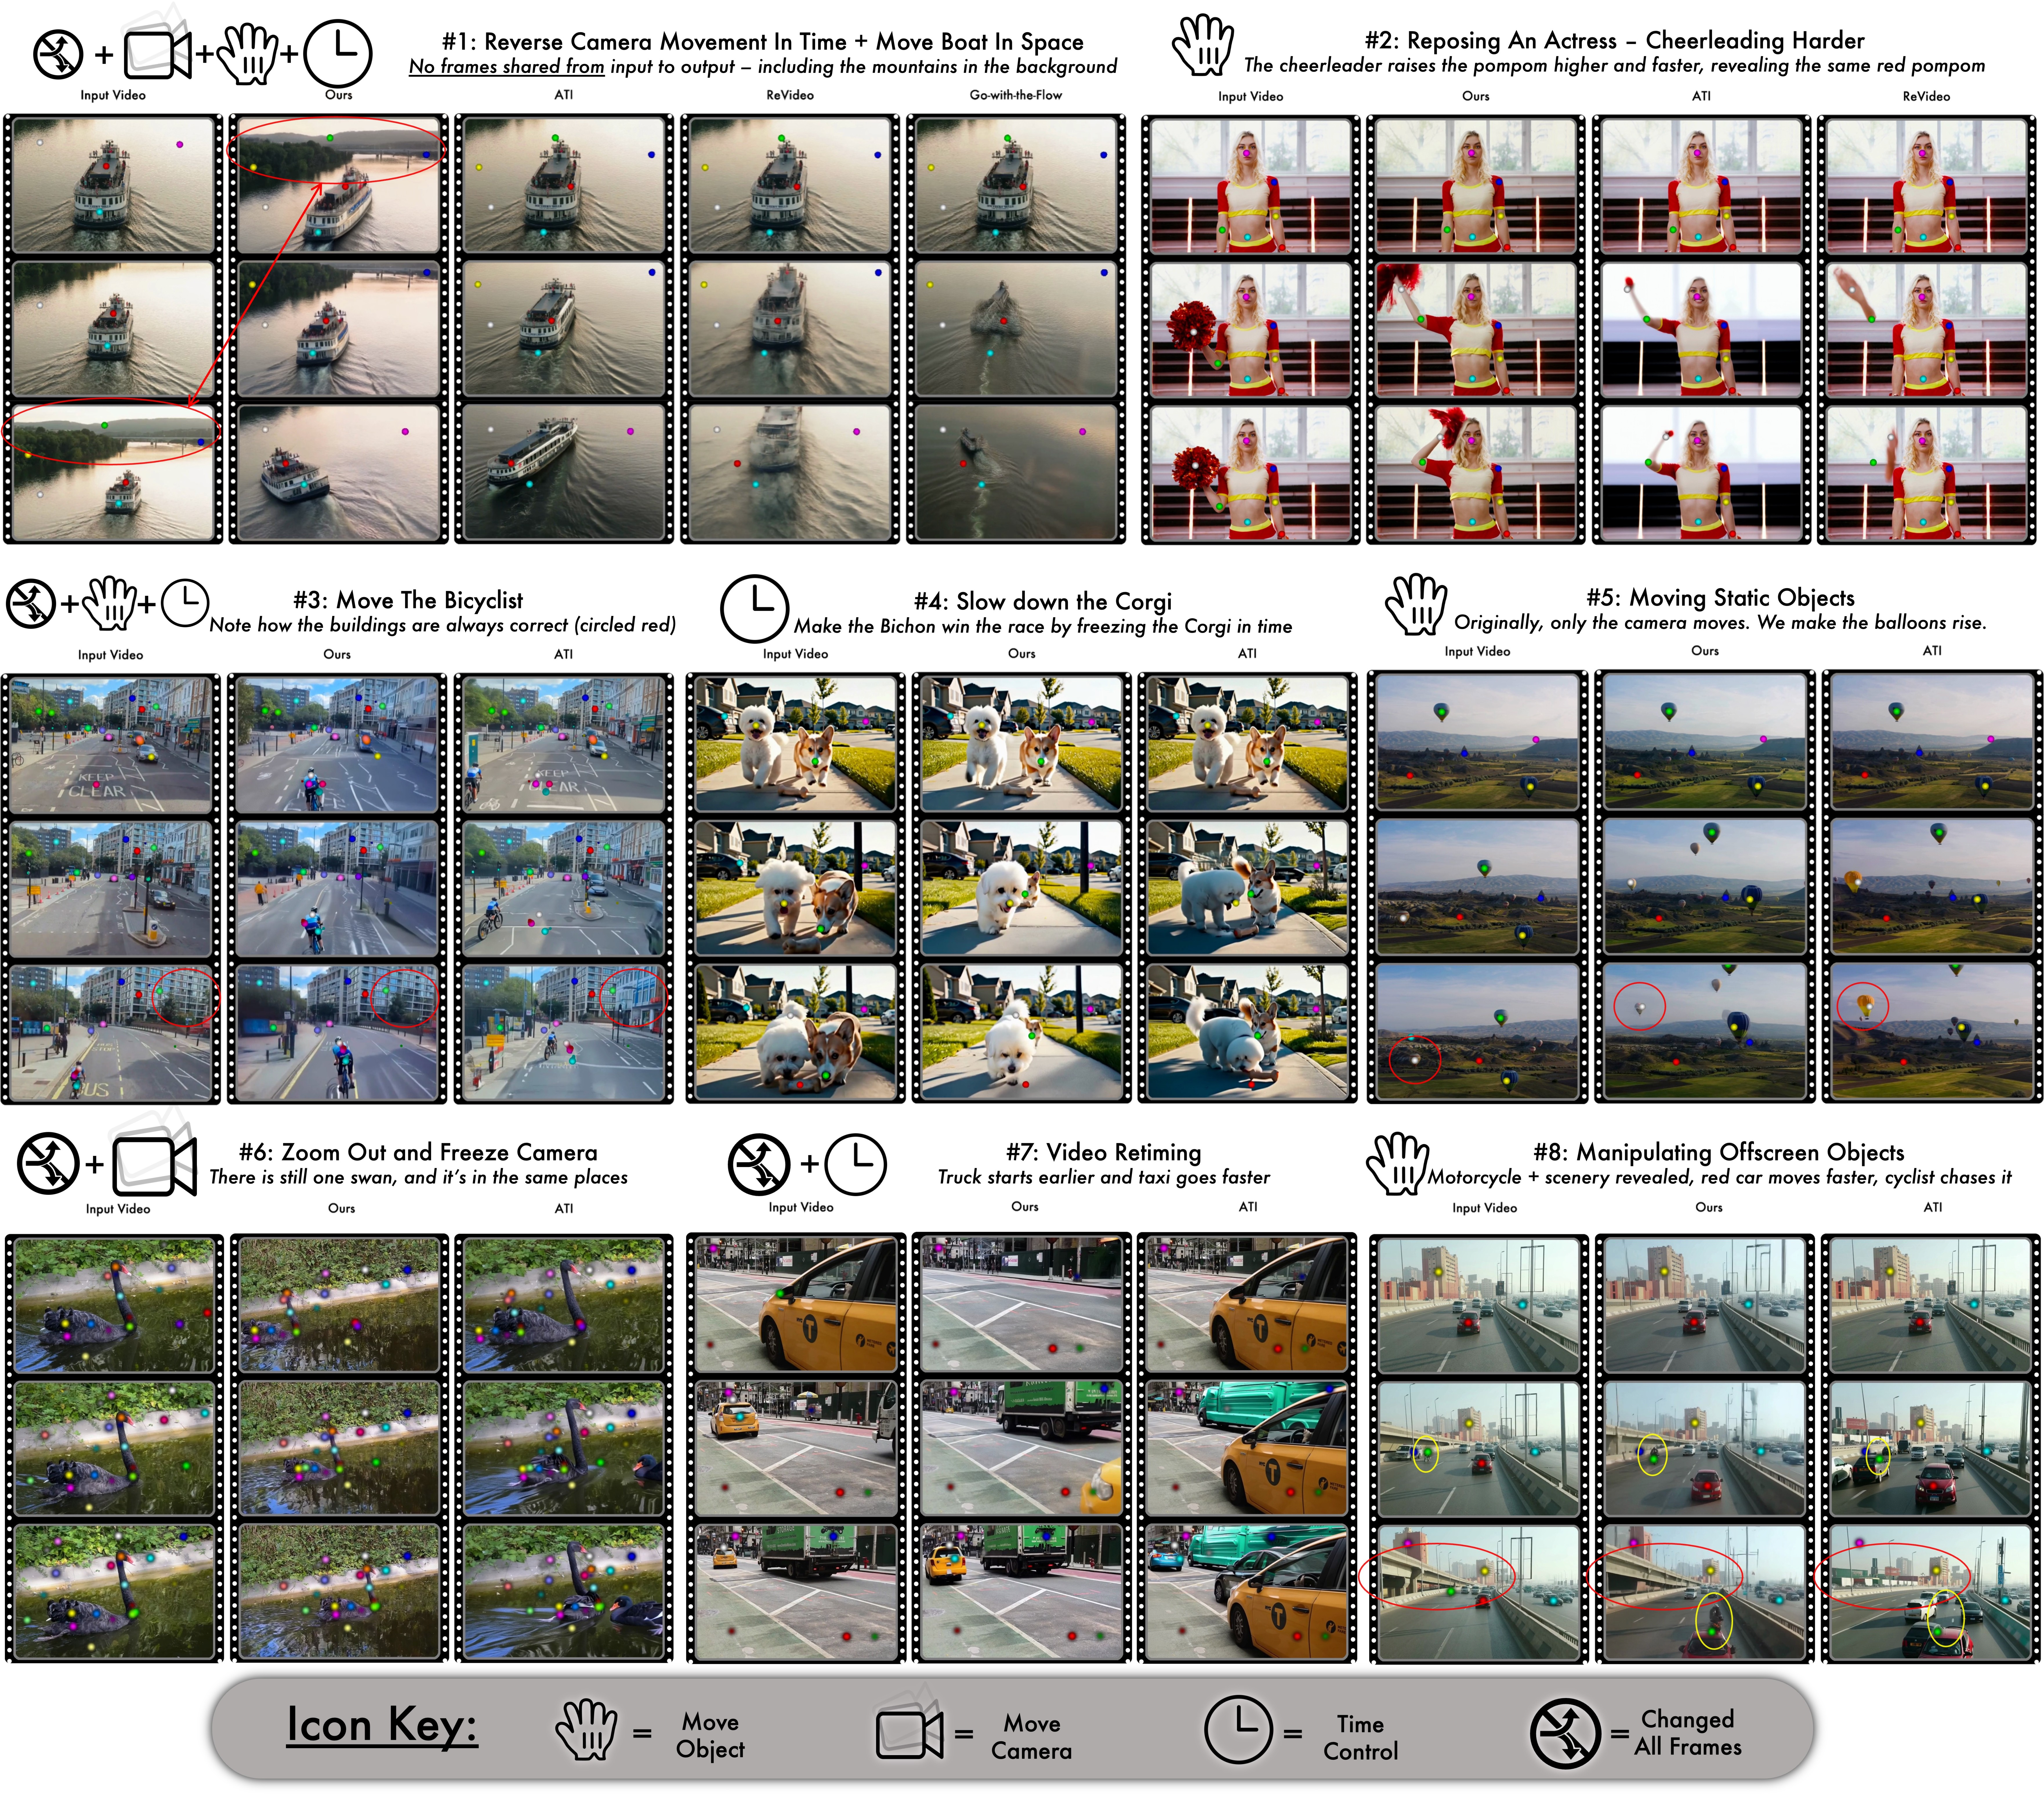
\includegraphics[width=1\linewidth]{megacomparisonfigurev2.jpg}
    % \includegraphics[width=1\linewidth]{\figfolder/MegaComparisonFigurev2}
    \caption{Comparison of our method vs.\ baselines across eight challenging motion editing scenarios.
Each row shows a different editing task with input video,
our result,
and ATI's result (with additional baselines shown for subfigure 4).
\textbf{Icon key:} Human Pose (modifying human motion),
Move Object (repositioning objects),
Move Camera (changing camera motion),
Time Control (retiming events),
Changed All Frames (no shared frames between input/output—impossible for image-to-video methods).
Colored dots track correspondence points throughout the video;
dot presence/absence indicates object visibility.
Red circles highlight key differences where baselines fail.}
    \label{fig:mega_comparison}
\end{figure*}

\noindent\textbf{Baseline comparisons.} Figure~\ref{fig:mega_comparison} compares our method against several baselines in multiple video editing scenarios, each of which demonstrate the capabilities of our motion edits. We primarily compare against ATI~\cite{ati},
a trajectory-guided image-to-video method based on WAN 2.1~\cite{wan},
our strongest baseline despite using a more powerful base model than our CogVideoX base.
Subfigure 4 additionally shows ReVideo~\cite{revideo2024} and Go-with-the-Flow~\cite{gowiththeflow2025},
which rated poorly in user evaluation—ReVideo lacks text conditioning and Go-with-the-Flow was not designed for point control.


\noindent\textbf{Edit \#1: Complex Edits on the Boat Scene.} This edit moves the boat left and shifts the camera so that mountains from the original's last frame appear in the edit's first. This requires specifying a substantial temporal trajectory change and holistic knowledge of the scene content. Ours is the only method that realistically moves the boat while correctly adjusting the camera to reveal the mountains at the beginning of the video.

\noindent\textbf{Edit \#2: Reposing a Cheerleader.} This edit raises the cheerleader's arms. The challenge involves preserving the red pom-pom, which is absent from the first frame. Ours successfully modifies the motion while retaining this content. In contrast, ATI and ReVideo rely solely on the first frame, leading to unnatural movements and a failure to preserve the pom-pom.

\noindent\textbf{Edit \#3: Move The Bicyclist.} This edit controls a cyclist visible only in the final frame of the original video. Ours correctly propagates the cyclist and tracking dots (cyan, magenta, white) throughout. ATI, lacking full temporal context, misplaces the cyclist and synthesizes wrong buildings (red circles).

\noindent\textbf{Edit \#4: Dog Race.}
Differential timing breaks single-frame-based methods. We decelerate the Corgi (green dot) to reverse the race outcome while keeping the Bichon steady. This requires independent temporal control; ATI fails to decouple the motions, incorrectly copying the Bichon and transforming a light pole into a tree.

\noindent\textbf{Edit \#5: Moving Static Balloons.}
We add upward motion to stationary balloons. The white balloon (white dot), which appears mid-video, challenges partial information methods. While ATI moves visible balloons, it renders the initially hidden white balloon orange due to missing appearance data. Our method uses full video context to maintain correct colors.

\noindent\textbf{Edit \#6: Zooming out on the Swan} 
In this DAVIS~\cite{davis2016} example, we transform a panning shot into a static, zoomed-out view. The output field of view differs entirely from the input, yet the swan must remain anchored to specific vegetation. Lacking full spatial context, ATI synthesizes a second swan and produces inconsistent motion.

\noindent\textbf{Edit \#7: Retiming a taxi.}
We do a complex isolated retiming of taxi and truck movement. This requires complete temporal understanding; ATI's single-frame generation cannot achieve this reversal. Figure~\ref{fig:mega_comparison} compares our method against ATI (WAN 2.1-based), as well as ReVideo and Go-with-the-Flow (in Subfigure 4), both of which were rated poorly due to their design limitations.

\noindent \textbf{Edit \#8: Moving an Offscreen Car.}
As the camera follows a red car, a motorcyclist enters late. We reposition this initially invisible rider behind the car while maintaining consistent background architecture. Lacking future frames to reference the rider and buildings (red circles), ATI synthesizes incorrect content.


\noindent\textbf{Discussion.}
These scenarios highlight I2V limitations: conditioning only on the first frame prevents leveraging information from the full input. Our V2V formulation enables bidirectional flow, allowing outputs to pull content from \emph{any} input frame. This handles offscreen content, camera changes, and reordering—challenges where I2V methods like ReVideo~\cite{revideo2024}, Go-with-the-Flow~\cite{gowiththeflow2025}, and MotionPrompting~\cite{motionprompt2024} fail.

% Additional comparison figures have been integrated into Figure~\ref{fig:mega_comparison}

%\begin{figure}[h]
%    \centering
%    \fullcompfig[1]{4}{\figfolder/FullComp_BlackSwan}
%    \caption{The camera is frozen while the black swan swims.}
%    \label{fig:comp_blackswan}
%\end{figure}
%
%\begin{figure}[h]
%    \centering
%    \fullcompfig[2]{5}{\figfolder/FullComp_Boat}
%    \caption{Editing the boat's trajectory and motion.\cih{todo: give categories / labels}}
%    \label{fig:comp_boat}
%\end{figure}
%
%\begin{figure}[h]
%    \centering
%    \fullcompfig[1]{4}{\figfolder/FullComp_Cheerleader}
%    \caption{Changing the motion of the cheerleader's pompoms.}
%    \label{fig:comp_cheerleader}
%\end{figure}
%
%\begin{figure}[h]
%    \centering
%    \fullcompfig[2]{4}{\figfolder/FullComp_Judge}
%    \caption{The judge walks in from the right with camera zoom.}
%    \label{fig:comp_judge}
%\end{figure}

%\begin{figure}[h]
%    \centering
%    \fullcompfig[1]{4}{\figfolder/FullComp_Candle}
%    \caption{A hand grabs the candle while the camera is stopped.}
%    \label{fig:comp_candle}
%\end{figure}

%\begin{figure}[h]
%    \centering
%    \fullcompfig[2]{4}{\figfolder/FullComp_CityBiker}
%    \caption{Editing the motion of an urban cyclist.\cih{a bit hard to see}}
%    \label{fig:comp_biker}
%\end{figure}
%
%\begin{figure}[h]
%    \centering
%    \fullcompfig[1]{4}{\figfolder/FullComp_Balloons}
%    \caption{Hot air balloons rise while the camera motion is slowed.}
%    \label{fig:comp_balloons}
%\end{figure}
%
%\begin{figure}[h]
%    \centering
%    \fullcompfig[1]{4}{\figfolder/FullComp_Dogs}
%    \caption{The corgi stays behind while the bichon moves forward.}
%    \label{fig:comp_dogs}
%\end{figure}

% \begin{figure}[h]
%     \centering
%     \includegraphics[width=1\linewidth]{\figfolder/FullComp_Shakycam}
%     \caption{Editing the camera motion on shaky footage. \cih{this just looks like brown}}    \label{fig:comp_shakycam}
% \end{figure}


\section{Conclusion}
\label{lss_sec:conclusion}

We introduce a novel language-based self-supervised learning (SSL) approach for videos, termed LSS, capable of adapting strong language-aligned image representations (CLIP \cite{radford2021clip}) to the video domain. 
In particular, we propose two self-distillation based SSL objectives, \textit{concept distillation} and \textit{concept alignment}.
Our approach trains with no video level labels or paired captions similar to prior video SSL works, but retains language alignment from image CLIP enabling direct zero-shot inference. We demonstrate state-of-the art performance in terms of linear probing with the learned representations on downstream tasks. For zero-shot operation, LSS demonstrates strong performance under both standard and transductive settings, indicating a promising direction for video SSL. 

\vspace{2em}
\noindent \textbf{Limitations, Future Work, \& Broader Impact}: 
The language alignment of LSS may be limited mostly to per-frame static information since the alignment is derived from image CLIP \cite{radford2021clip}. LSS cannot distinguish motion based categories like \texttt{"moving object left to right"}. Moreover, while containing highly discriminative and generic information at image level, CLIP features lack spatial awareness at an object level \cite{ranasinghe2022perceptual}. Our proposed model building off these representations in inherently limited in understanding object level motion and interaction within videos. However, recent progress in localization aware CLIP models \cite{ranasinghe2022perceptual,Xu2023LearningOS,xu2022groupvit} opens avenues for leveraging their object-centric or pixel-level representations to better model such video motion patterns, opening up interesting future directions. 
In terms of broader impact, the datasets and pre-trained models we use possibly contain biases, which may be reflected in LSS. However, our reduced reliance on human annotations may lower additional biases.

% % \vspace{-0.5em}
% \textbf{Reproducibility Statement}: 
% We build a codebase derived from source code of SVT \cite{Ran2021SVT} \& CLIP \cite{radford2021clip} and use pre-trained CLIP weights from \texttt{https://github.com/openai}. All experiments use publicly available datasets. Our action descriptions will be released publicly along with our codebase.

% \textbf{Acknowledgements}:
% We thank Xiang Li for helpful discussions and server setup. We also thank Kumara Kahatapitiya and Cristina Mata for helpful discussions.

\clearpage
{
    \small
    \bibliographystyle{ieeenat_fullname}
    \bibliography{main}
}

% WARNING: do not forget to delete the supplementary pages from your submission
\clearpage
%\setcounter{page}{1}
\maketitlesupplementary

\section{Gaussianity preservation of our noise warping algorithm}

In this section, we discuss our noise warping algorithm, providing a formal proof of its Gaussianity preservation properties. We also present an illustrative example that demonstrates how noise that undergoes expansion and subsequent contraction returns to its original state, showcasing how our noise warping algorithm maintains the underlying Gaussian distribution throughout the warping process.

\begin{proof}
    For each $(x,y) \in V$, $R(x,y)$ is a collection of upsampled noise $X_i$, where
    \begin{align*}
    \bE[X_i] &= \bE[\frac{q(x,y)}{d}] + \bE[\frac{1}{\sqrt{d}}(Z_i - \frac{S}{d})] = 0  \\
        \Var(X_i) &= \Var(\frac{q(x,y)}{d}) + \Var(\frac{1}{\sqrt{d}}(Z_i - \frac{S}{d})) \\
        &= \frac{1}{d^2} + \frac{1}{d} \Var(\frac{d-1}{d}Z_i - \sum_{j\neq i} \frac{Z_j}{d}) \\
        &= \frac{1}{d^2} + \frac{1}{d} \frac{(d-1)^2 + (d-1)}{d^2} = \frac{1}{d},
    \end{align*}
    where we used the fact that $q(x,y)$ and $Z_i$'s are i.i.d. standard Gaussians.
    Since $X_i$ is constructed as a weighted sum of Gaussians, itself is also a Gaussian.
    Moreover, for $i \neq j$, we compute
    \begin{align*}
        &\Cov(X_i, X_j) \\
        =&\Cov(\frac{q(x,y)}{d} + \frac{1}{\sqrt{d}}(Z_i - \frac{S}{d}), \frac{q(x,y)}{d} + \frac{1}{\sqrt{d}}(Z_j - \frac{S}{d})) \\
        =& \frac{1}{d^2} + \frac{1}{d}\bE[(Z_i - \frac{S}{d})(Z_j - \frac{S}{d})] \\
        =& \frac{1}{d^2} + \frac{1}{d}(0 - 2 \frac{\bE[Z_i S]}{d} + \frac{\bE[S^2]}{d^2}) \\
        =& \frac{1}{d^2} + \frac{1}{d}(-\frac{2}{d} + \frac{1}{d}) = 0.
    \end{align*}
    Hence all $X_i$'s are independent.

    For each $(x',y') \in V'$, if $\deg_G((x',y')) = 0$, then $q'(x',y')$ is sampled as an independent standard Gaussian. 
    Otherwise, the output noise pixel $q'(x',y')$ is built as a weighted sum of $R(x,y)\text{.pop}()$ for each edge $((x,y), (x',y'))\in E$, where $R(x,y)\text{.pop}()$ is an independent Gaussian of mean 0 and variance $\frac{1}{\deg_G((x,y))}$.
    Hence $q'(x',y')$ is also a Gaussian with mean 0.
    The variable $s$ after executing the inner for loop thus represents the variance of $q'(x',y')$, so the renormalization at the end brings $q'(x',y')$ back to a standard Gaussian.
    Since the composing $X_i$'s are independent, the resulting noise $q'$ should also have an independent Gaussian in each pixel.
\end{proof}

\begin{example}[Exact recovery of \expansion-\contraction]
Consider the following evolution of noise across three frames with forward flows $f_{i\to j}$ going from frame $i$ to frame $j$ with $i + 1 = j$ (and backward flow if $i -1 = j$).
Suppose at frame $1$, a pixel $v \in D$ with density $1$ has noise $q$. Suppose further that $v'_a$ is a pixel at frame $2$ such that $f_{1\to 2}^{-1}(v'_a) = \{v\}$, and $v'_b \in D$ is the only pixel at frame $2$ such that $f_{1\to 2}^{-1}(v_b') = \varnothing$ and $f_{2\to 1}(v'_b) = v$.
This represents the scenario where $v$ is expanded into two pixels $v'_a,v'_b$.
Then \cref{alg:main} with forward flow $f_{1\to 2}$ and backward flow $f_{2 \to 1}$ will result in $v'_a$ having density $1/2$ and noise $\frac{q}{2} + \frac{1}{\sqrt{2}}(\frac{Z_a-Z_b}{2})$, and $v_b'$ having density $1/2$ and noise $\frac{q}{2} + \frac{1}{\sqrt{2}}(\frac{Z_b-Z_a}{2})$, where $Z_a$ and $Z_b$ are i.i.d. standard Gaussians.
Now, from frame $2$ to frame $3$, suppose there exists a pixel $v''$ such that $f_{2\to 3}^{-1}(v'') = \{v'_a,v'_b\}$, i.e., they both $v'_a$ and $v'_b$ contract to $v''$, and that $f_{3\to2}(D) \cap \{v'_a,v'_b\} = \varnothing$.
Then \cref{alg:main} with forward flow $f_{2\to 3}$ and backward flow $f_{3\to 2}$ will result in $v''$ having density $1$ and noise $q$, hence deterministically recovering the noise and density of $v$ in frame 0.

\end{example}


\section{Qualitative results of training-free image diffusion based video editing}

Noise warping methods that do not preserve Gaussianity degrade per-frame performance, as originally pointed out in~\cite{chang2024warped}. For example, using nearest neighbor and bilinear interpolation destroys the Gaussianity (see \cref{fig:supp_warped_noise_flow_vis}) and consequently deteriorates the per-frame performance on pre-trained image-to-image diffusion models (see \cref{fig:supp_davis_deepfloyd} and \cref{fig:supp_diffrelight_noisewarp}).

\begin{figure*}
    \centering
    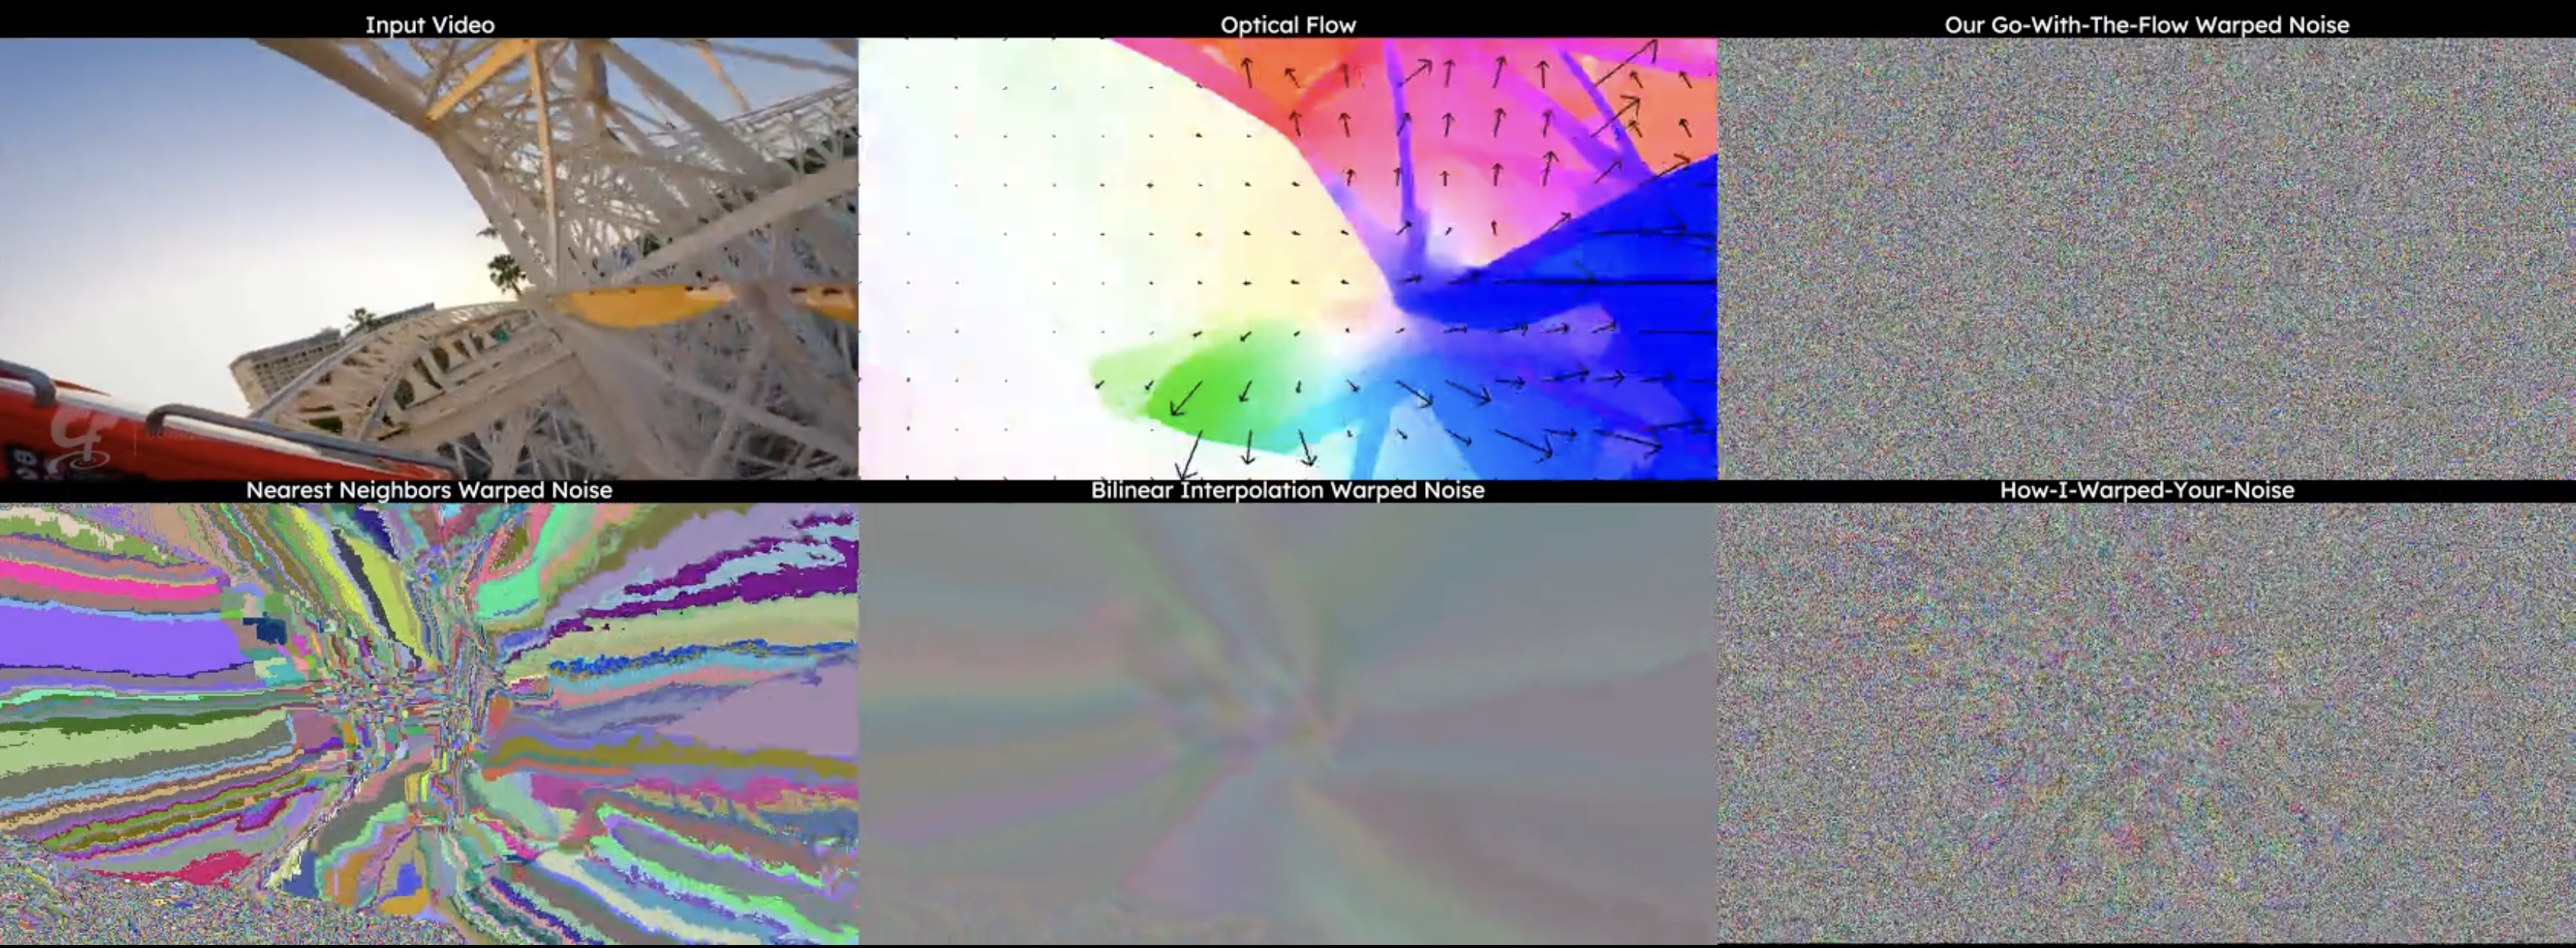
\includegraphics[width=1\linewidth]{fig/nongauss_vis.png}
    \caption{A direct visualization of the noise produced by our noise warping algorithm, HIWYN~\cite{chang2024warped}, bilinear, and nearest neighbor interpolations. The forward movement in this long roller-coaster video forces the noise to expand significantly. Early in the video, the HIWYN baseline produces visibly non-Gaussian results. See the full video on our \href{https://eyeline-research.github.io/Go-with-the-Flow/}{webpage}.}
    \label{fig:supp_warped_noise_flow_vis}
\end{figure*}

\begin{figure}
    \centering
    \includegraphics[width=1\linewidth]{fig/stroller_frame20.png}
    \caption{Using different noise warping algorithms on DeepFloyd~IF for video super-resolution on the DAVIS dataset.}
    \label{fig:supp_davis_deepfloyd}
\end{figure}

\begin{figure}
    \centering
    \includegraphics[width=1\linewidth]{fig/naz_diffrelight_grid11.jpg}
    \caption{Using different noise warping algorithms on DifFRelight for portrait video relighting. }
    \label{fig:supp_diffrelight_noisewarp}
\end{figure}


\section{The advantage of noise warping}

By using noise warping as a condition for motion, we effectively discard all structural information from our input video that cannot be inferred from motion alone. This can be advantageous, as demonstrated in \cref{fig:supp_windmill}. MotionClone does not use optical flow to guide the video trajectory, instead relying on manipulating activations within the diffusion model. As a result, the windmill gains an extra set of arms, whereas our method, which relies solely on motion information from optical flow via warped noise, does not introduce such artifacts.

\section{Comparison to the video diffusion base model without finetuning}

Interestingly, video diffusion models respond to noise warping even without training. In \cref{fig:supp_windmill} the rightmost column, even though the per-frame quality suffers, the flow of the output video still roughly follows the flow of the warped noise. However, because warped noise is statisically distinct from the pure Gaussian noise CogVideoX was trained on, without fine-tuning it can result in visual artifacts.

\section{User study settings and statistics}
\label{sec:supp_user_study}

\cref{fig:supp_user_study_screenshots_statistics} presents our user study questionnaires and statistics for two applications: (1) local object motion control, and (2) turnable camera movement video generation. Our questions focus on users' overall subjective preference, controllability, and temporal consistency.

\section{Model Agnostic}


Our method is data- and model-agnostic. It can be used to add motion control to arbitrary video diffusion models by only processing the noise sampling during fine-tuning. For example, it also works with AnimateDiff \cite{guo2024animatediff} fine-tuned on the WebVid dataset~\cite{Bain21} (the weights for this model on our \href{https://github.com/Eyeline-Research/Go-with-the-Flow}{GitHub} page). See its qualitative results in \cref{fig:supp_animatediff_grid}. Since release, the community has also trained a version of Go-with-the-Flow on HunyuanVideo (linked on our \href{https://github.com/Eyeline-Research/Go-with-the-Flow}{GitHub} page). Therefore, our method will generalize to future more advanced video diffusion base model.

\section{Pseudo code}

See \cref{listing:supp_algo_pseudo_code} for our noise warping pseudo code. See our source code and model checkpoints on \href{https://github.com/GoWithTheFlowPaper/gowiththeflowpaper.github.io}{GitHub}.

\begin{figure*}
    \centering
    \includegraphics[width=0.7\linewidth]{fig/windmills.pdf} 
    \caption{
    We show a \cutndrag~animation of a windmill rotating clockwise, next to the derived optical flow, our outputs, a baseline and an ablation. \textbf{Note} that the input video column appears to have two sets of panels because it's being cut and dragged over itself to create rotational motion. \textbf{When using noise warping is better}: Per-frame structural information can poison the result of MotionClone, giving the windmill an extra set of arms - whereas ours only receives motion information from optical flow alone via warped noise (there are no double-windmills in the optical flow patterns). \textbf{Ablation in rightmost column}: warped noise with $\deglevel=.5$ on the CogVideoX base model before we fine-tune it. Because warped noise is statisically distinct from the pure Gaussian noise CogVideoX was trained on, without fine-tuning it can result in visual artifacts. Note how although the per-frame quality suffers here, it still picks up on motion queues from the warped noise (the camera zooms into the windmill).}
    \label{fig:supp_windmill}
\end{figure*}

\begin{figure*}
    \centering
    \begin{subfigure}{.48\linewidth}
    \includegraphics[width=\linewidth]{fig/user_study_screenshot_1.png}
    \subcaption{User study interface and questions for local object motion control, corresponding to ~\cref{fig:comparisons_video_diffusion_object_motions} in the main paper.}
    \end{subfigure}
    \hfill
    \begin{subfigure}{.48\linewidth}
    \includegraphics[width=\linewidth]{fig/user_study_screenshot_2.png}
    \subcaption{User study interface and questions for turnable camera movement video generation, corresponding to ~\cref{fig:comparisons_video_diffusion_turning_object} in the main paper.}
    \end{subfigure}
    \\[12pt]
    \begin{subfigure}{0.48\linewidth}
    \centering
    \includegraphics[width=.7\linewidth]{fig/user_study_1_statistics_1.png}
    \subcaption{User study statistics for local object motion control on the first question ``\textit{Which video is the best overall?}''}
    \end{subfigure}
    \hfill
    \begin{subfigure}{0.48\linewidth}
    \centering
    \includegraphics[width=.7\linewidth]{fig/user_study_1_statistics_2.png}
    \subcaption{User study statistics for local object motion control on the second question ``\textit{Which video best aligns with the user intent for controlling the object movement based on the input?}''}
    \end{subfigure}
    \\[12pt]
    \begin{subfigure}{0.48\linewidth}
    \centering
    \includegraphics[width=.7\linewidth]{fig/user_study_1_statistics_1.png}
    \subcaption{User study statistics for local object motion control on the third question ``\textit{Which video best preserves the intended camera movement from the input?}''}
    \end{subfigure}
    \hfill
    \begin{subfigure}{0.48\linewidth}
    \centering
    \includegraphics[width=.7\linewidth]{fig/user_study_1_statistics_1.png}
    \subcaption{User study statistics for local object motion control on the fourth question ``\textit{Which video maintains the most consistent and stable motion throughout?}''}
    \end{subfigure}
    \\[12pt]
    \begin{subfigure}{0.48\linewidth}
    \centering
    \includegraphics[width=0.7\linewidth]{fig/user_study_2_statistics_1.png}
    \subcaption{User study statistics for motion transfer on the first question ``\textit{Which video has better overall quality?}''}
    \end{subfigure}
    \caption{User study questionnaires screenshots and statistics. For all the questions of both applications, our method (the rightmost bar plot) significantly wins the most user preferences.}
    \label{fig:supp_user_study_screenshots_statistics}
\end{figure*}

% \begin{figure*}
%     \centering
%     \includegraphics[width=1\linewidth]{fig/animatediff.jpg}
%     \caption{Fine-tuning AnimateDiff with our warped noise flow. All rows share the same movements, and all columns share the same text prompts. The first column is the reference video providing the flow to warp the noise in column 2, which is then used to diffuse all videos to the right. Please zoom in to see the captions for each row (input videos driving movement and warping noise via optical flow) and each column (text prompt for each video cell). Refer to our project video to see these in animation form.}
%     \label{fig:supp_animatediff_grid}
% \end{figure*}

\begin{figure*}
    \centering
    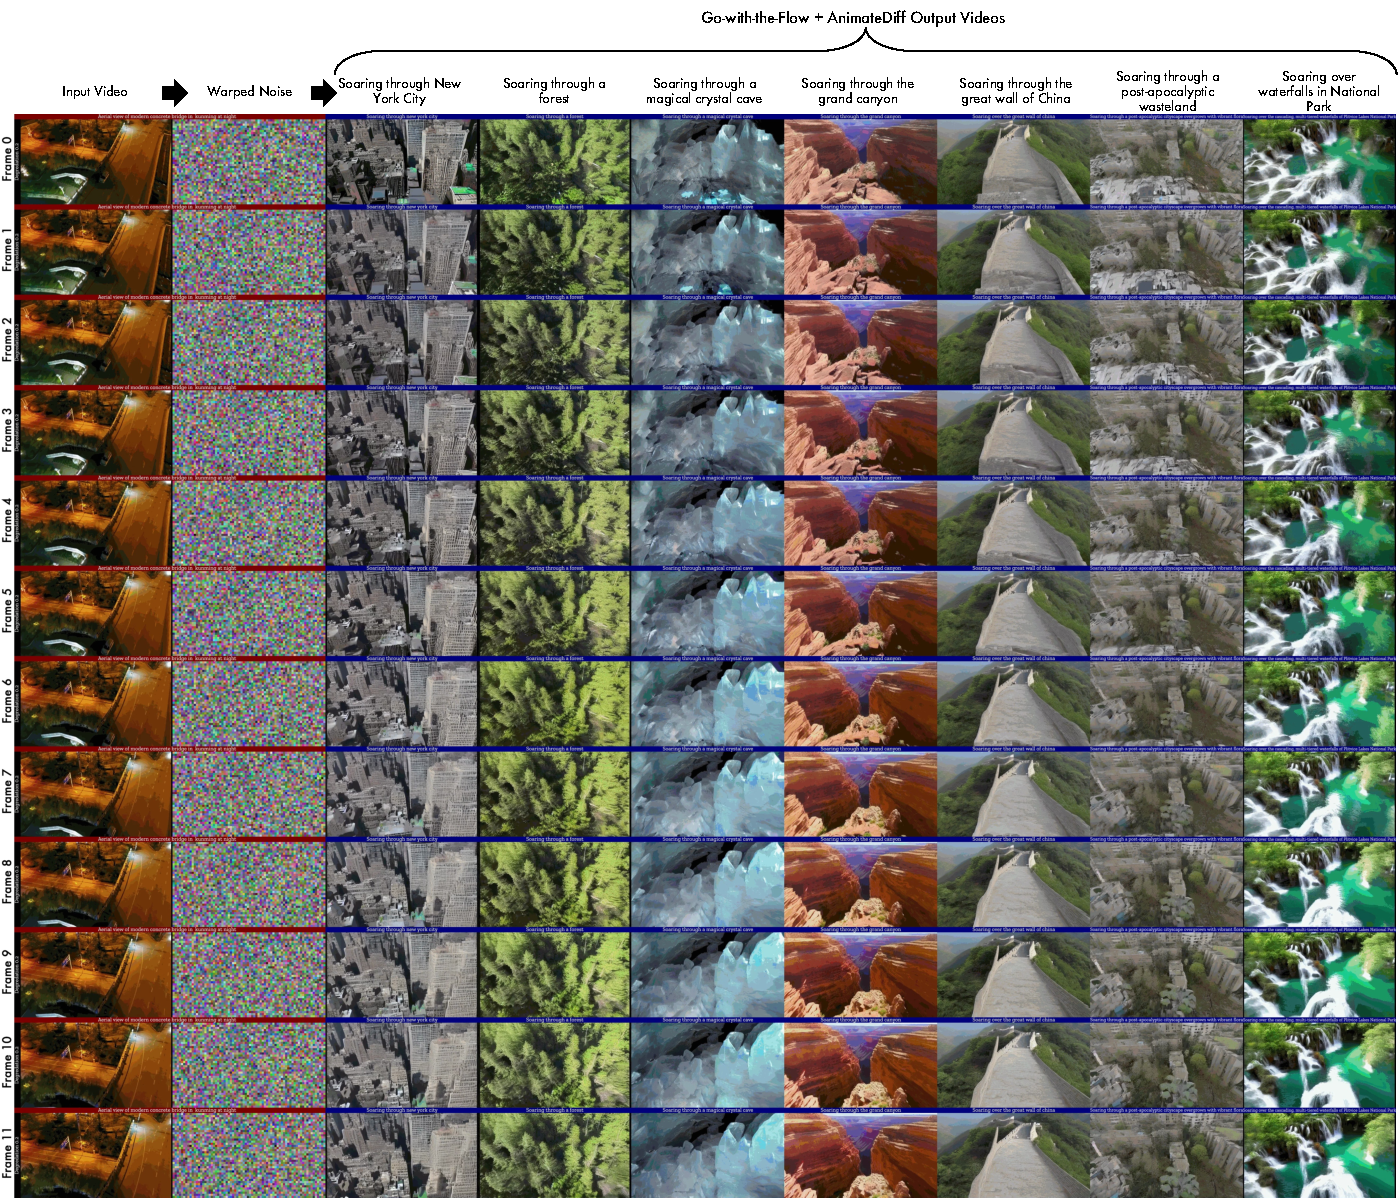
\includegraphics[width=1\linewidth]{fig/AnimateDiffAnimation.pdf}
    \caption{Fine-tuning AnimateDiff with our warped noise flow. We used Go-with-the-Flow to fine-tune AnimateDiff T2V, and display the results above. The input video is on the left, and from that video we derive warped noise which is used to initialize AnimateDiff on the columns to its right with different text prompts.}
    \label{fig:supp_animatediff_grid}
\end{figure*}

\begin{figure*}
\begin{lstlisting}
def warp_noise(prev_frame, cur_frame, prev_noise, prev_weight):

    height, width, _ = prev_frame.shape

    flow = optical_flow(prev_frame, cur_frame) # Agnostic to the optical flow algorithm
    backwards_flow = -flow # A cheap approximation of optical_flow(cur_frame, prev_frame)

    expansion_noise    = zeros(height, width)
    contraction_noise  = prev_noise.copy()

    expansion_mask     = ones (height, width, type=bool)
    contraction_mask   = zeros(height, width, type=bool)

    for x in range(width): for y in range(height):
        dx, dy = flow[x,y]
        if 0 <= x+dx <= width-1 and 0 <= y+dy <= height-1:
            # This particle stays in bounds
            expansion_mask  [x+dx, y+dx] = False
            contraction_mask[x   , y   ] = True  # Contraction mask is True where 

    for x in range(width): for y in range(height):
        if expansion_mask[x, y]:
            dx, dy = backwards_flow[x,y]
            expansion_noise [x, y] = prev_noise[x+dx, y+dy]

    # We've decided which source pixels are involved in contraction and expansion now
    contraction_noise &= contraction_mask
    expansion_noise, contraction_noise, cur_weight = jointly_regaussianize_and_rebalance_weights(
        expansion_noise, contraction_noise, prev_weight
    ) # Regaussianize all noise values here, and divide the weights by the number of pixels in each bin

    contraction_weight = zeros(height, width)
    for x in range(width): for y in range(height):
        if contraction_mask[x, y]:
            # Contraction treats the noise pixels as particles, each moving from the source to the
            # destination with this flow
            dx, dy = flow[x,y]
            # Contraction is a weighted sum of source pixels to a destination pixel
            pixel_weight = cur_weight[x, y]
            # Sum all the source noise pixels that contract to the same destination
            contraction_noise [x+dx, y+dy] += prev_noise[x, y] * pixel_weight
            # When we multiply a noise pixel by a weight, the variance changes by that weight squared
            contraction_weight[x+dx, y+dy] += pixel_weight ** 2 
    contraction_noise /= sqrt(contraction_weight) # Adjust the variance of the summed contracted noise

    # Mixing contraction and expansion noises with their respective masks
    cur_noise = contraction_noise & contraction_mask + expansion_noise & expansion_mask

    return cur_noise, cur_weight
\end{lstlisting}
\caption{Our noise warping pseudo code.}
\label{listing:supp_algo_pseudo_code}
\end{figure*}


\end{document}